\section{Poisson Arrivals See Time Averages}
\label{sec:poisson-arrivals-see}

\subsection*{Theory and Exercises}

\Opensolutionfile{hint}
\Opensolutionfile{ans}

Suppose the following limit exists:
\begin{equation}\label{eq:jaap}
  \pi(n) 
= \lim_{m\to\infty} 
\frac1m\sum_{k=1}^m \1{L(A_k-) = n},
\end{equation}
where $\pi(n)$ is the long-run fraction of jobs that observe $n$
customers in the system at the moment of arrival.  It is natural to
ask whether $\pi(n)$ and $p(n)$, as defined by~\eqref{eq:p(n)}, are related, that is, whether what
customers see upon arrival is related to the time-average behavior of
the system. In this section we will derive the famous \recall{Poisson arrivals see time averages (PASTA)} condition  that ensures that  $\pi(n)=p(n)$ if the arrivals follow a Poisson process. 


\begin{comment}
\begin{hint}
Check the definitions of $Y(0,t)$, $Y(1,t)$, $A(0,t)$ and so on. Make a drawing of $Y(0, t)$ and $Y(1,t)$ as functions of $t$. 
\end{hint}
  \begin{solution}
 $A(t)=\lfloor t\rfloor$ provided the unit of $t$ is in
  hours. $A(0,t)=A(t)$ and $A(n,t)=0$ for $n>0$.  Next, for $Y(0,t)$ we define, for notational ease, the fractional part of $t$ as $\{t\} = t - \lfloor t \rfloor$. Then,
  \begin{align*}
    Y(0,t)&= \frac 1{60} \lfloor t \rfloor + \{t\} \1{ \{t\} \in[59/60, 1)} \approx \frac{1}{60}t, \\
    Y(1,t)&= \frac{59}{60} \lfloor t \rfloor + \{t\} \1{\{t\}\in[0,59/60)} \approx \frac{59}{60}t. \\
\lambda(0) &= \lim_t \frac{A(0,t)}{Y(0,t)} = \lim_t \frac{t}{t/60} = 60, \\
\lambda(1) &= \lim_t \frac{A(1,t)}{Y(1,t)} = \lim_t\frac{0}{59/60 t} = 0 \\
\lambda(n) &= 0, \quad n\geq 1. \\
\lambda &= \lim_t \frac{A(t)}t  = 1 \\
p(0)  &= \frac{1}{60}, \\
p(1)  &= \frac{59}{60}, \\
\rho  &= \frac{59}{60}, \\
\pi(0)  &= 1. \\
  \end{align*}
  There is no queue so $\E{L_Q} = 0$, but $\E L = \rho$.  The queue
  length as observed by customers is equal to 0, because jobs only
  arrive when the server is free.
  \end{solution}
\end{exercise}
  \end{comment}

\begin{comment}
\begin{exercise}
 Consider another (theoretical) queueing system in which each
  customer requires precisely 1 minute. At the start of each hour, 59
  customers arrive. What is $p(n)$, what is $\pi(n)$? What is the time-average system length $\E{L}$?
  \begin{solution}
As in the previous problem, $\rho=59/60$.

For $p(n)$: the fraction of time the system contains $n=0$ jobs is $p(0)=1/60=1-\rho$. Also, as the service time of each job is precisely one minute, $p(n)=1/60$ for $n=1,\ldots, 59$. 

For $\pi(n)$, the first of the $59$ jobs sees a free server, thus $\pi(0)=1/59$. The second job of the $59$ jobs sees one job in system (and this job is in service), hence $\pi(1)=1/59$. More generally then, $\pi(n)=1/59$ for $n=0,\ldots 58$. 

Note in particular $p(59)=1/60 \neq \pi(59) = 0$. 

  Observe now that the average system length is very different from the
  previous example, even though $\rho = 59/60$ in both cases. Thus,
  knowledge of the load is not sufficient to make a statement about the
  average queue length.

  To compute the average queue length, as perceived by the customers,
  note that the first customer sees no queue, the second sees one
  customer in front, and so on. Thus, the average queue length as seen
  by customers is
  \begin{equation*}
   \frac{0+1+2+\cdots+58}{59}=\frac{1}{59}\frac{58\cdot 59}{2} = 29.
  \end{equation*}
The time average system length is $\E L = 59/60 + 58/60 + \cdots 1/60 + 0/60 = 59/2$. 
  \end{solution}
\end{exercise}
\end{comment}

We can make some progress by rewriting $\pi(n)$ in
the following way. Since $A(t)\to \infty$ as $t\to\infty$, it is reasonable 
that\footnote{See below for the proof.}
\begin{equation}\label{eq:132}
  \begin{split}
  \pi(n) &= \lim_{t\to\infty} \frac1{A(t)}\sum_{k=1}^{A(t)} \1{L(A_k-) = n} \\
  &= \lim_{t\to\infty} \frac1{A(t)}\sum_{k=1}^\infty \1{A_k \leq t, L(A_k-) = n} \\
  &= \lim_{t\to\infty} \frac{A(n,t)}{A(t)},
  \end{split}
\end{equation}
where we use~\eqref{eq:19} in the last row. But, 
\begin{equation}\label{eq:1333}
 \frac{A(n,t)}{t} 
= \frac{A(t)}t \frac{A(n,t)}{A(t)}
\to \lambda  \pi(n), \quad\text{as } t \to \infty, 
\end{equation}
where we use Eq.~\eqref{eq:3}, i.e., $A(t)/t \to \lambda$. 
Next, by  Eq.~\eqref{eq:21}, 
\begin{equation*}
\frac{A(n,t)}t = \frac{A(n,t)}{Y(n,t)}\frac{Y(n,t)}t \to \lambda(n) p(n), \quad\text{as } t \to \infty.
\end{equation*}
Thus
\begin{equation}\label{eq:13}
\lambda  \pi(n) = \lambda(n) p(n), 
\end{equation}
from which  follows our final result:
\begin{equation*}
  \lambda(n) = \lambda \iff \pi(n) = p(n), 
\end{equation*}

\begin{exercise}\label{ex:8} Show that for the case of Exercises~\ref{ex:111} and~\ref{ex:112} $\pi(0)=1$ and $\pi(n)=0$, for $n>0$.

\begin{solution}
  All arrivals see an empty system. Hence $A(0,t)/A(t) \approx (t/2)/(t/2) = 1$, and $A(n,t)=0$ for $n>0$. Thus, $\pi(0) = \lim_t A(0,t)/A(t) = 1$ and $\pi(n)=0$ for $n>0$. Recall from the other exercises that $p(0)=1/2$. Hence, time average statistics are not the same as statistics at arrival moments. 
\end{solution}

\end{exercise}

\begin{exercise}
  Check that~(\ref{eq:13})  holds for the system of Exercise~\ref{ex:8}.
  \begin{solution}
From the relevant previous exercises, $\lambda = \lim_t A(t)/t = 1/2$. $\lambda(0)=1$, $p(0)=1/2$, and $\pi(0)=1$. Hence,
\begin{equation*}
  \lambda \pi(0) = \lambda(0) p(0) \implies  \frac 1 2 \times 1 = 1\times \frac 1 2.
\end{equation*}
For $n>0$ it's easy, everything is 0.
  \end{solution}
\end{exercise}


So, why is this useful? Well, in words, it means that if the arrival
rate does not depend on the state of the system, i.e.,
$\lambda=\lambda(n)$, the sample average $\pi(n)$ is equal to the
time-average $p(n)$, i.e., $\pi(n)=p(n)$. But, when $\pi(n)=p(n)$, the
customer perception at arrival moments, i.e., $\pi(n)$, is the same as
the server perception, i.e., $p(n)$.

As the exercises above show, this property is not satisfied in
general.  However,  when the arrival process is
Poisson we have that $\lambda(n)=\lambda$. This fact is typically called \recall{PASTA:
  Poisson Arrivals See Time Averages}. Thus, when customers arrive in
accordance to a Poisson process (hence the inter-arrival times are
exponentially distributed), it must be that $\pi(n) = p(n)$, and
for the $M/M/1$ queue,
\begin{equation*}
  \pi(n) = p(n) = (1-\rho)\rho^n.
\end{equation*}


With the above reasoning, we can also establish a relation between
$\pi(n)$ and the statistics of the system as obtained by the
departures. For this we
turn again to Eq.~\eqref{eq:15}, i.e., $|A(n,t) - D(n,t)| \leq 1$. To
obtain Eq.~\eqref{eq:12} we divided both sides of this equation by the
time the system spends in a certain state. We can also use another
form:
\begin{equation*}
\frac{A(t)}t \frac{A(n,t)}{A(t)} = \frac{A(n,t)}t \approx \frac{D(n,t)}t 
= \frac{D(t)}t \frac{D(n,t)}{D(t)}.
\end{equation*}
Taking limits at the left and right, we see again that the left hand
becomes $\lambda \pi(n)$. For the right hand side, we use
Eq.~\eqref{eq:28} and define, analogous to \eqref{eq:132}, 
\begin{equation}
  \label{eq:33}
  \delta(n) = \lim_{t\to\infty} \frac{D(n,t)}{D(t)}.
\end{equation}
Thus, $\delta(n)$ is the long-run fraction of jobs that leave $n$ jobs
\emph{behind}. Clearly, then, if the limits exist, the right hand side
tends to $\delta \delta(n)$ as $t\to\infty$. Hence, for (queueing)
systems in which customers arrive and leave as single units, we have
\begin{equation}
  \label{eq:36}
  \lambda \pi(n) = \delta \delta(n).
\end{equation}
Moreover, if the system is rate-stable, i.e., the output rate $\delta$ is equal to the input rate $\lambda$, we obtain
\begin{equation}
  \label{eq:39}
\lambda = \delta \iff  \pi(n) = \delta(n).
\end{equation}
This means that the system as seen by arrivals, i.e., $\pi(n)$, is
the same as what jobs leave behind, i.e., $\delta(n)$.


\begin{exercise}\label{ex:26}
  When $\lambda\neq \delta$, is $\pi(n)\geq \delta(n)$ or $\pi(n) < \delta(n)$ true?  (This is a tricky exercise!) 
  \begin{hint}
    Use that    $\lambda \geq \delta$ always holds. Thus, when $\lambda \neq \delta$, it must be that $\lambda > \delta$. What are the consequences of this inequality; how does the queue length behave as a function of time?
  \end{hint}
  \begin{solution}
    The assumptions lead us to conclude that $\lambda > \delta$. As a consequence, the queue length must increase on the long run (jobs come in faster than they leave). Therefore, $A(n,t)/t \to 0$ for all $n$, and also $D(n,t)/t\to 0$. Consequenly, $\pi(n) = \delta(n) = 0$, which is the only sensible reconciliation with~\eqref{eq:36}. 
  \end{solution}
\end{exercise}

\begin{exercise}
Show that 
\begin{equation*}
\lambda  \pi(n) = \lambda(n) p(n) = \mu(n+1) p(n+1) = \delta \delta(n).
\end{equation*}
What is the important condition for this to be true?
\begin{hint}
Check all definitions of $Y(n,t)/t$ and so on.
\end{hint}
\begin{solution}
  The important condition is that transitions occur as single
  steps. In other words, the relation is true for processes with
  \recall{one-step transitions}, i.e., when $|A(n,t) - D(n,t)|\leq 1$.
  In  that case, 
\begin{align*}
  \frac{A(n,t)}{t} &=   \frac{A(n,t)}{A(t)} \frac{A(t)}{t} \to \pi(n) \lambda\\
  \frac{A(n,t)}{t} &=   \frac{A(n,t)}{Y(n,t)} \frac{Y(n,t)}{t} \to \lambda(n)p(n)\\
  \frac{D(n,t)}{t} &=   \frac{D(n,t)}{Y(n+1,t)} \frac{Y(n+1,t)}{t} \to \mu(n+1)p(n+1)\\
  \frac{D(n,t)}{t} &=   \frac{D(n,t)}{D(t)} \frac{D(t)}{t} \to \delta(n)\delta. \\
\end{align*}
\end{solution}
\end{exercise}



\begin{exercise}
  Why is $\mu(n) = \mu$ for the $M/M/1$ queue?  
  \begin{hint}
Think about the
    construction of the $M/M/1$ queue as a random walk, see
    Section~\ref{sec:queu-proc-as}.
  \end{hint}
 \begin{solution}
   The $M/M/1$-queue can be constructed as a reflection of the random
   walk $Z(t) = Z(0) + N_\lambda(t) - N_\mu(t)$. Clearly,
   down crossings can only occur when $N_\mu$ fires. The rate at which
   the transitions of $N_\mu$ occur is constant, and, in particular,
   independent of the history of $Z$. 

   More specifically, for the interested, define
   $\sigma\{X(t) : t\in I\}$ as the $\sigma$-algebra generated by the
   stochastic processes $\{X(t), t\in I\}$ on the index set $I$. Then,
   by construction of $\{N_\lambda(t)\}$ and $\{Z(t)\}$, we have that
   $\sigma\{Z(s) : s\in[0,t]\}$  and $\sigma\{N_\lambda(u) : u > t\}$ are independent.
 \end{solution}
\end{exercise}


\begin{exercise}
  Use the PASTA property and the ideas of Section~\ref{sec:level-cross-balance}
 to derive for the $M/M/1$ queue that
$(\lambda + \mu) \pi(n) = \lambda \pi(n-1) + \mu \pi(n+1)$.
  \begin{hint}
    Consider some state $n$ (not a level) and count all transitions that `go in and
    out of' this state. Specifically, $A(n,t) + D(n-1,t)$ counts all
    transitions out of state $n$: $A(n,t)$ counts the number of
    arrivals that see $n$ in the system upon arrival, hence
    immediately after such arrivals the system contains $n+1$ jobs;
    likewise, $D(n-1,t)$ counts all jobs that leave $n-1$ jobs behind,
    hence immediately before such jobs depart the system contains $n$
    jobs.  In a similar way, $A(n-1,t) + D(n,t)$ counts all
    transitions into state $n$ (Recall once again, $D(n,t)$ counts the
    jobs that leave $n$ behind. Hence, when such departures occur,
    state $n$ is entered). Now use that `what goes in must go out'.    
  \end{hint}
  \begin{solution}
By  the hint,  the difference between the `out
    transitions' and the `in transitions' is at most 1 for all $t$. Thus,  we can write
    \begin{align*}
\text{transitions out } &\approx \text{transitions in } \iff \\
      A(n,t) + D(n-1,t) &\approx A(n-1,t) + D(n,t)  \iff \\
      \frac{A(n,t) + D(n-1,t)}t &\approx \frac{A(n-1,t) + D(n, t)}t \iff \\
      \frac{A(n,t)}t + \frac{D(n-1,t)}t &\approx \frac{A(n-1,t)}t + \frac{D(n,t)}t.
    \end{align*}
Using the ideas of Section~\ref{sec:level-cross-balance} this becomes for $t\to\infty$, 
\begin{equation*}
  (\lambda(n) +\mu(n))p(n) = \lambda(n-1)p(n-1) + \mu(n+1)p(n+1).
\end{equation*}
Since we are concerned here with the $M/M/1$ queue we have that
$ \lambda(n) = \lambda$ and $\mu(n) = \mu$, and using PASTA we have
that $p(n) = \pi(n)$. We are done.
  \end{solution}
\end{exercise}



There is a subtle problem in the transition from~\eqref{eq:jaap} to~\eqref{eq:132} and the derivation
of~\eqref{eq:1333}: $\pi(n)$ is defined as a limit over arrival epochs
while in $A(n,t)/t$ we take the limit over time. Now the observant
reader might ask why these limits should relate at all.  The
resolution lies in the \recall{renewal reward theorem}. This
theorem is very useful in its own right, and states  intuitively that 
when customers arrive at rate $\lambda$ and each customer pays an average amount $X$, then the system earns money at rate $Y=\lambda X$.  Figure~\ref{fig:renewal} provides graphical motivation about why this theorem is true; \citet{el-taha98:_sampl_path_analy_queuein_system}
gives  a (simple) proof.

\begin{theorem}[Renewal Reward Theorem, $Y=\lambda X$]
  Suppose the counting process $\{N(t), t\geq 0\}$ is such that
  $N(t)/t\to\lambda$ as $t\to\infty$, where $0<\lambda < \infty$. Let
  $\{Y(t), t\geq 0\}$ be a non-decreasing right-continuous
  (deterministic) process. Define $X_k = Y(T_k)-Y(T_{k-1})$,
  $k\geq 1$, where $T_k$ are the epochs at which $N$ increases, i.e.,
  $N(t) = \{k : T_k \leq t\}$. Then $Y(t)/t$ has a limit iff
  $n^{-1}\sum_k^n X_k$ has a limit in which case $Y=\lambda X$, i.e.,
  \begin{equation*}
  \lim_{t \to \infty} \frac{Y(t)}t=Y \iff \lim_{n \to \infty} \frac 1n\sum_k^n X_k =X \implies Y=\lambda X.
  \end{equation*}
\end{theorem}

\begin{figure}[ht]
  \centering
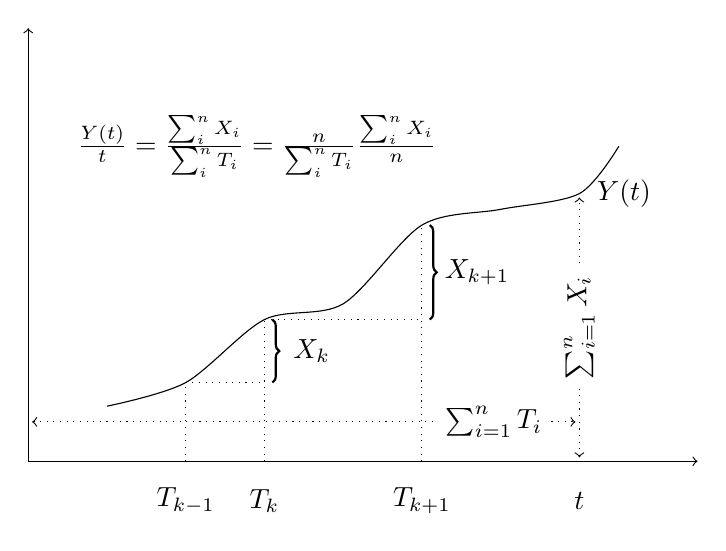
\begin{tikzpicture}[scale=1]
%axis
\draw[->] (0,0) -- coordinate (x axis mid) (8.5,0);
\draw[->] (0,0) -- coordinate (y axis mid) (0,5.5);
%\node[below=0.2cm] at (x axis mid) {$t$};

\draw plot [smooth] coordinates {(1,0.7) (2,1) (3,1.8) (4,2) (5,3) (6,3.2) (7, 3.4) (7.5,4.0)};
\node[right]  at (7.1,3.4) {$Y(t)$};
\node  at (7.,-0.5) {$t$};

\node  at (2.,-0.5) {$T_{k-1}$};
\draw[dotted] (2,0)--(2,1);
\draw[dotted] (2,1)--(3,1);


\node  at (3.,-0.5) {$T_{k}$};
\draw[dotted] (3,0)--(3,1.8);
\draw[dotted] (3,1.8)--(5,1.8);

\draw [
    thick,
    decoration={brace, mirror, raise=0.1cm },
    decorate
] (3,1) -- (3,1.8)
node[pos=0.5, xshift=0.6cm]  {$X_k$}; 


\node  at (5.,-0.5) {$T_{k+1}$};
\draw[dotted] (5,0)--(5,3);

\draw [
    thick,
    decoration={brace, mirror, raise=0.1cm },
    decorate
] (5,1.8) -- (5,3)
node[pos=0.5, xshift=0.7cm]  {$X_{k+1}$}; 

\node[right] at (0.5,4) {$\frac{Y(t)}t = \frac{\sum_i^n X_i}{\sum_{i}^n T_i} = \frac{n}{\sum_{i}^n T_i} \frac{\sum_i^n X_i}n $};


\draw[dotted,<->, =stealth] (7,0.05)--(7,3.35) node[midway, rotate=90, fill=white] {$\sum_{i=1}^n X_i$};
\draw[dotted,<->, =stealth] (0.05,0.5)--(6.95,0.5) node[pos=0.85, fill=white] {$\sum_{i=1}^n T_i$};
\end{tikzpicture}
\caption{A graphical `proof' of $Y=\lambda X$. Here $Y(t)/t\to Y$, $n/\sum^n_i T_i\to \lambda$ and $n^{-1}\sum_i^n X_i \to X$.  (Observe that in the
  figure $X_k$ does not represent an inter-arrival time; instead it
  corresponds to the increment of (the graph of) $Y(t)$ between two
  consecutive epochs $T_{k-1}$ and $T_k$ at which $Y(t)$ is
  observed.) }
  \label{fig:renewal}
\end{figure}


\begin{exercise}
Use the renewal reward theorem to show that~(\ref{eq:132}) is valid.
\begin{hint}
Check that the conditions of the renewal reward theorem are satisfied in the above proof~\eqref{eq:1333}. Then define  
\begin{align*}
  Y(t) &:= A(n,t) = \sum_{k=1}^{A(t)} \1{L(A_k-) = n} \\
X_k &:= Y(A_k) - Y(A_{k-1}) = A(n, A_k) - A(n, A_{k-1}) = \1{L(A_k-)=n}.
\end{align*}

\end{hint}
\begin{solution}
First we check the conditions.  The counting process here is $\{A(t)\}$ and the epochs at which
    $A(t)$ increases are $\{A_k\}$. By assumption, $A_k\to\infty$,
    hence $A(t)\to\infty$ as $t\to\infty$. Moreover, by assumption
    $A(t)/t \to \lambda$. Also $A(n,t)$ is evidently non-decreasing and
    $A(n,t)\to\infty$ as $t\to\infty$.


From the definitions in the hint,   
\begin{equation*}
X= \lim_{m\to\infty} \frac 1 m \sum_{k=1}^m X_k =\lim_{m\to\infty} \frac 1 m \sum_{k=1}^m \1{L(A_k-)=n} = \pi(n).
\end{equation*}
Since $Y=\lim_t Y(t)/t = \lim_t A(n,t)/t$ it follows from the renewal reward theorem that
\begin{equation*}
  Y=\lambda X \implies \lim_t \frac{A(n,t)} t = \lambda X = \lambda \pi(n).
\end{equation*}
Thus, Eq.~\eqref{eq:1333} follows from the renewal reward theorem.
\end{solution}
\end{exercise}



With the PASTA property we can determine the distribution
of the inter-departure times of the $M/M/1$ queue.  We will need these
results when we analyze networks of queues---observe that in a network
of queues the departures from one queueing station form the arrivals
at another station. We chop up this problem into small steps to help you
find the answer mostly by yourself.


\begin{exercise}\label{ex:dep}
Why is the output rate of the (stable) $M/M/1$ queue equal to~$\lambda$ and not~$\mu$?
\begin{solution}
Jobs arrive at rate $\lambda$. For a stable queue, $\mu>\lambda$. Moreover,  jobs can never leave faster than they arrive.
\end{solution}
\end{exercise}


\begin{exercise}
Why is $\mu e^{-\mu t}$ not a reasonable density for the
    inter-departure times?
    \begin{solution}
         Because jobs do not leave at rate $\mu$. 
    \end{solution}
\end{exercise}

The simplest guess for the inter-departure density might be $\lambda e^{-\lambda t}$; so this is what we will try to prove. As we will see, this result holds. 

We will focus on departure moments and use~\eqref{eq:39}, in particular that departures `see' what arrivals `see', i.e., $\delta(n)= \pi(n)$, and PASTA.


\begin{exercise}
 Observe that when a customer departs, the server can be either
    idle $I$ or busy $B$.   Show that $\P{I} = 1-\rho$.
    \begin{solution}
 $\P I = p(0) =\pi(0)=\delta(0)$.  Recall now that $p(0) = 1-\rho$.
    \end{solution}
\end{exercise}

\begin{exercise}\label{ex:17}
 If job $n-1$, say, leaves behind an empty system, show that the expected time until the next departure is $\E{D_n - D_{n-1}} = 1/\lambda + 1/\mu$. 
    \begin{hint}
      After job $n-1$ left, job $n$ has to arrive, so we need to wait first for this inter-arrival time. Then job $n$ must be served. This adds up to $1/\lambda + 1/\mu$. 
    \end{hint}
    \begin{solution}
With the hint, we first have to wait for an inter-arrival
    time $X_n$. Then, since job $n$'s service starts right away, it
    leaves when $D_n = D_{n-1}+X_n + S_n$. Now observe that, due to the memoryless property of the inter-arrival times, $\E{X_n} = \E{A_n - D_{n-1}} = 1/\lambda$. Thus, the expected duration is $\E{X_n + S_n}=1/\lambda + 1/\mu$. 
    \end{solution}
\end{exercise}

\begin{exercise}
Show that the density of $D_{n} - D_{n-1}$ is
    \begin{equation*}
    f_{X+S}(t) = \frac{\lambda \mu}{\lambda - \mu} (e^{-\mu t} - e^{-\lambda t})
    \end{equation*}
if the server is idle after $D_{n-1}$.
    \begin{solution}
      By the previous point, the density of $D_{n} - D_{n-1}$ is the
      same as the density of $X_n + S_n$.  Since $\{X_n\}$ and $\{S_n\}$ are both i.i.d. sequences, the problem becomes to find the density of $X+S$.  We will use two ways of computing this. 

\newpage
Since $X\sim \Exp(\lambda)$ and $S\sim\Exp(\mu)$, and $X$ and $S$ are independent, their joint density is $f_{X,S}(x,y) = \lambda \mu e^{-\lambda x - \mu y}$. With this,
  \begin{align*}
\P{X+S\leq t } 
&= \lambda \mu \int_0^\infty \int_0^\infty e^{-\lambda x - \mu y} \1{x+y\leq t} \d x \d y \\
&= \lambda \mu \int_0^t \int_0^{t-x} e^{-\lambda x - \mu y} \d x \d y \\
&= \lambda \mu \int_0^t e^{-\lambda x} \int_0^{t-x} e^{- \mu y} \d y \d x \\
&= \lambda \int_0^t e^{-\lambda x} (1-e^{- \mu (t-x)} ) \d x  \\
&= \lambda \int_0^t e^{-\lambda x}  \d x - \lambda e^{-\mu t} \int_0^t e^{(\mu-\lambda) x} \d x \\
&= 1- e^{-\lambda t} - \frac{\lambda}{\mu-\lambda} e^{-\mu t} ( e^{(\mu-\lambda) t} -1) \\
&= 1- e^{-\lambda t} - \frac{\lambda}{\mu-\lambda} e^{-\lambda t} + \frac{\lambda}{\mu-\lambda} e^{-\mu t} \\ 
&= 1 - \frac{\mu}{\mu-\lambda} e^{-\lambda t} + \frac{\lambda}{\mu-\lambda} e^{-\mu t}. \\
  \end{align*}
The density $f_{X+S}(t)$ is the derivative of this expression with respect to~$t$, hence,
\begin{align*}
  f_{X+S}(t) 
&= \frac{\lambda\mu}{\mu-\lambda} e^{-\lambda t}  - \frac{\mu \lambda}{\mu-\lambda} e^{-\mu s} \\
&= \frac{\lambda\mu}{\lambda -\mu}(e^{-\mu t} - e^{-\lambda t}). \\
\end{align*}

Conditioning is much faster, but requires the concept of conditional density. You can skip the rest if you are not interested. 
    \begin{align*}
    f_{X+S}(t) 
&= \P{X+S\in \d{t}} \\
&= \int \P{S+x\in \d{t}}\P{X\in \d{x}} \\
&=\int_0^t f_S(t-x) f_X(x) \d{x} \\
     &= \int_0^t \mu e^{-\mu(t-x)} \lambda e^{-\lambda x} \d{x} \\
     &= \lambda \mu e^{-\mu t} \int_0^t  e^{x(\mu-\lambda)} \d{x} \\
& \frac{\lambda \mu}{\lambda - \mu} (e^{-\mu t} - e^{-\lambda t}).
    \end{align*}
    \end{solution}
\end{exercise}

\begin{exercise}
Show that the probability that a job leaves behind a busy station is $\rho$.
    \begin{solution}
For the time average, 
        $\P B = \sum_{n=1}^\infty p(n) = \rho$.
    \end{solution}
From PASTA $\pi(n) = p(n)$, hence the fraction of jobs that see a busy server must be $\rho$. Finally, as $\delta(n) = \pi(n)$, a fraction $\rho$ of the departures leaves a busy system behind.
\end{exercise}

\begin{exercise}
Show  that when the server is busy at $D_{n-1}$, the density of the inter-departure time is $f_D(t) = \mu e^{-\mu t}$.
    \begin{solution}
The server can start right away with a new job. The departure times are exponentially distributed. 
    \end{solution}
\end{exercise}

\begin{exercise}
Use conditioning on the server being idle or busy at a departure to show that  the density of  the inter-departure time is $\lambda e^{-\lambda t}$.
  \begin{hint}
Conditioning leads to 
\begin{equation*}
    f_D(t) = f_{X+S}(t) \P{I} + f_S \P B = (1-\rho) f_{X+S}(t) +
    \rho \mu e^{-\mu t}.
\end{equation*}
    Now use the above exercises to simplify.
  \end{hint}
  \begin{solution}
       \begin{align*}
    f_D(t) 
&= f_{X+S}(t) \P I + f_S \P B \\
&= (1-\rho) f_{X+S}(t) +    \rho \mu e^{-\mu t} \\
&= (1-\rho) \frac{\mu\lambda}{\lambda-\mu} \left(e^{-\mu t}-e^{-\lambda t}\right) +    \rho \mu e^{-\mu t} \\
&= \left(1-\frac{\lambda}\mu\right) \frac{\mu\lambda}{\lambda-\mu}\left(e^{-\mu t}-e^{-\lambda t}\right)  +    \rho \mu e^{-\mu t} \\
&= \frac{\mu-\lambda}\mu \frac{\mu\lambda}{\lambda-\mu}\left(e^{-\mu t}-e^{-\lambda t}\right)  +    \frac\lambda \mu \mu e^{-\mu t} \\
% &= \frac{\mu-\lambda}\mu \frac{\mu\lambda}{\lambda-\mu}\left(e^{-\mu t}-e^{-\lambda t}\right)  +    \lambda e^{-\mu t} \\
&= - \lambda\left(e^{-\mu t}-e^{-\lambda t}\right)  +    \lambda e^{-\mu t} \\
&=  \lambda e^{-\lambda t}.
      \end{align*}
  \end{solution}
\end{exercise}

It can also be shown that the inter-departure times are independent. 

\begin{exercise}\label{ex:burke}
Explain that the above leads to \recall{Burke's law}  which states that the departure process of the $M/M/1$ queue is a Poisson  process with rate $\lambda$. 
\begin{solution}
The above exercises show that inter-departures times have the same density, i.e., $\lambda e^{-\lambda t}$. The remark above states these times are independent. Thus,  the inter-departures times form a set of i.i.d. exponentially distributed random variables with mean $1/\lambda$. Consequently, the departures times form a Poisson process with rate $\lambda$.
\end{solution}
\end{exercise}




\Closesolutionfile{hint}
\Closesolutionfile{ans}

\opt{solutionfiles}{
\subsection*{Hints}
\input{hint}
\subsection*{Solutions}
\input{ans}
}
%\clearpage


%%% Local Variables:
%%% mode: latex
%%% TeX-master: "../queueing_book"
%%% End:
